% =============================================================================
% STAR UI Implementation Primer
% Comprehensive Guide for Vue 3 Progressive Web App
% =============================================================================

\documentclass[11pt,letterpaper]{article}

\usepackage[utf8]{inputenc}
\usepackage[T1]{fontenc}
\usepackage{geometry}
\usepackage{graphicx}
\usepackage{hyperref}
\usepackage{listings}
\usepackage{xcolor}
\usepackage{fancyhdr}
\usepackage{titlesec}
\usepackage{booktabs}
\usepackage{longtable}
\usepackage{tabularx}
\usepackage{enumitem}
\usepackage{tikz}
\usepackage{float}

\usetikzlibrary{shapes.geometric, arrows.meta, positioning}

\geometry{margin=1in}

\hypersetup{
    colorlinks=true,
    linkcolor=blue!70!black,
    urlcolor=cyan!70!black,
    pdftitle={STAR UI Implementation Primer},
}

\definecolor{codebg}{RGB}{245,245,245}
\definecolor{codeframe}{RGB}{200,200,200}
\definecolor{codekey}{RGB}{0,0,180}
\definecolor{codecomment}{RGB}{0,128,0}
\definecolor{codestring}{RGB}{163,21,21}

\lstset{
    basicstyle=\ttfamily\small,
    backgroundcolor=\color{codebg},
    frame=single,
    rulecolor=\color{codeframe},
    breaklines=true,
    tabsize=2,
    showstringspaces=false,
    numbers=left,
    numberstyle=\tiny\color{gray},
    keywordstyle=\color{codekey}\bfseries,
    commentstyle=\color{codecomment}\itshape,
    stringstyle=\color{codestring},
}

\lstdefinelanguage{TypeScript}{
    keywords={const, let, var, function, return, if, else, for, while, class, interface, type, export, import, from, async, await, new, this, extends, implements, static, public, private, protected, readonly, enum, namespace, module, declare, typeof, instanceof, in, of, as, is, keyof, infer, never, unknown, any, void, null, undefined, true, false, try, catch, finally, throw, switch, case, default, break, continue, do, debugger, delete, with, yield, get, set, constructor},
    morekeywords=[2]{string, number, boolean, object, symbol, bigint, Array, Promise, Map, Set, Record, Partial, Required, Readonly, Pick, Omit, Exclude, Extract, NonNullable, ReturnType, Parameters, InstanceType},
    keywordstyle=[2]\color{codecomment},
    morecomment=[l]{//},
    morecomment=[s]{/*}{*/},
    morestring=[b]',
    morestring=[b]",
    morestring=[b]`,
    sensitive=true,
}

\pagestyle{fancy}
\fancyhf{}
\fancyhead[L]{\leftmark}
\fancyhead[R]{STAR UI Primer}
\fancyfoot[C]{\thepage}

\title{\textbf{STAR UI Implementation Primer}\\[0.5cm]
\large Vue 3 + TypeScript Progressive Web App}
\author{STAR Development Team}
\date{December 2025}

\begin{document}

\maketitle
\tableofcontents
\newpage

% =============================================================================
\section{Project Overview}
% =============================================================================

\subsection{Purpose}

The \texttt{star-ui} is a Progressive Web App (PWA) for controlling and monitoring the STAR robot. It provides:

\begin{itemize}
    \item \textbf{Real-time Dashboard} with telemetry visualization
    \item \textbf{Map View} with live SLAM visualization
    \item \textbf{Motor Control} via gRPC-Web for low-latency commands
    \item \textbf{Offline Support} with service workers and IndexedDB
    \item \textbf{Installable} as native-like app on mobile devices
\end{itemize}

\subsection{Technology Stack}

\begin{table}[H]
\centering
\begin{tabular}{|l|l|l|}
\hline
\textbf{Component} & \textbf{Technology} & \textbf{Version} \\
\hline
Framework & Vue 3 & 3.4.x \\
Language & TypeScript & 5.x \\
Build Tool & Vite & 5.x \\
State Management & Pinia & 2.x \\
GraphQL Client & Apollo Client & 3.x \\
gRPC Client & gRPC-Web & 1.x \\
PWA & Workbox & 7.x \\
Styling & Tailwind CSS & 3.x \\
\hline
\end{tabular}
\caption{Technology Stack}
\end{table}

\subsection{Architecture}

\begin{figure}[H]
\centering
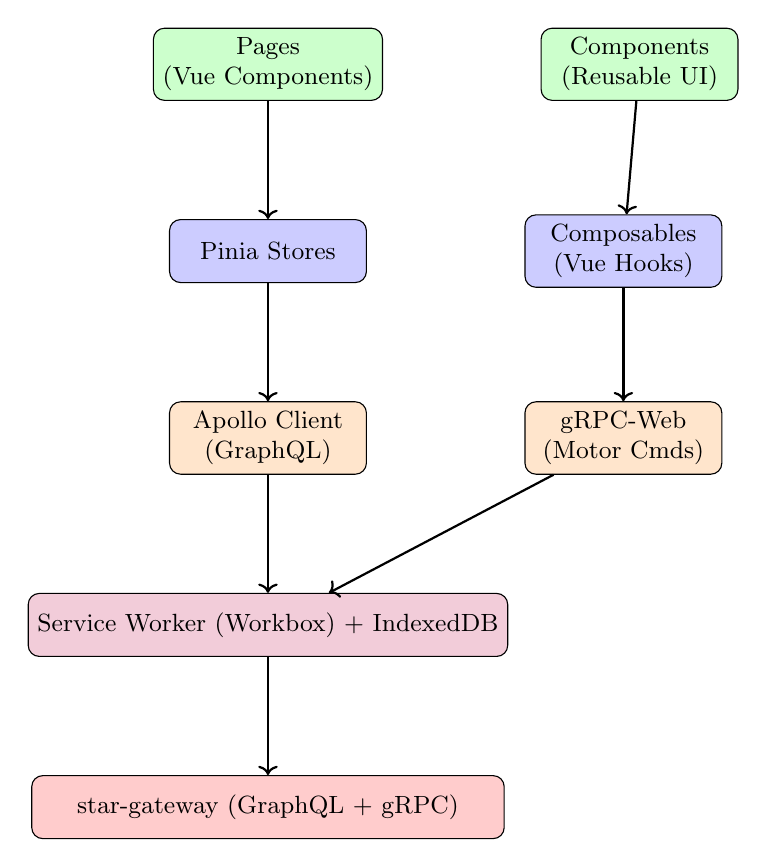
\begin{tikzpicture}[
    node distance=1.2cm,
    box/.style={draw, rectangle, rounded corners, minimum width=2.5cm, minimum height=0.8cm, align=center, font=\small},
    arrow/.style={->, thick}
]
    % UI Layer
    \node[box, fill=green!20] (pages) {Pages\\(Vue Components)};
    \node[box, fill=green!20, right=2cm of pages] (components) {Components\\(Reusable UI)};

    % State Layer
    \node[box, fill=blue!20, below=1.5cm of pages] (pinia) {Pinia Stores};
    \node[box, fill=blue!20, right=2cm of pinia] (composables) {Composables\\(Vue Hooks)};

    % Data Layer
    \node[box, fill=orange!20, below=1.5cm of pinia] (apollo) {Apollo Client\\(GraphQL)};
    \node[box, fill=orange!20, right=2cm of apollo] (grpc) {gRPC-Web\\(Motor Cmds)};

    % Service Worker
    \node[box, fill=purple!20, below=1.5cm of apollo, minimum width=6cm] (sw) {Service Worker (Workbox) + IndexedDB};

    % Backend
    \node[box, fill=red!20, below=1.5cm of sw, minimum width=6cm] (gateway) {star-gateway (GraphQL + gRPC)};

    % Connections
    \draw[arrow] (pages) -- (pinia);
    \draw[arrow] (components) -- (composables);
    \draw[arrow] (pinia) -- (apollo);
    \draw[arrow] (composables) -- (grpc);
    \draw[arrow] (apollo) -- (sw);
    \draw[arrow] (grpc) -- (sw);
    \draw[arrow] (sw) -- (gateway);
\end{tikzpicture}
\caption{Frontend Architecture}
\end{figure}

% =============================================================================
\section{Project Structure}
% =============================================================================

\begin{lstlisting}[language=bash]
star-ui/
|-- package.json
|-- vite.config.ts
|-- tsconfig.json
|-- tailwind.config.js
|-- index.html
|
|-- public/
|   |-- manifest.json             # PWA manifest
|   |-- icons/                    # App icons (192x192, 512x512)
|   +-- robots.txt
|
|-- src/
|   |-- main.ts                   # App entry point
|   |-- App.vue                   # Root component
|   |-- router/
|   |   +-- index.ts              # Vue Router config
|   |
|   |-- pages/
|   |   |-- DashboardPage.vue     # Main dashboard
|   |   |-- MappingPage.vue       # SLAM visualization
|   |   |-- ControlPage.vue       # Manual control
|   |   |-- SensorsPage.vue       # Sensor data
|   |   |-- SettingsPage.vue      # Configuration
|   |   +-- AnalyticsPage.vue     # Mission stats
|   |
|   |-- components/
|   |   |-- TelemetryCard.vue
|   |   |-- ImuVisualization.vue
|   |   |-- BatteryIndicator.vue
|   |   |-- MapCanvas.vue
|   |   |-- VirtualJoystick.vue
|   |   |-- ConnectionStatus.vue
|   |   +-- EventLog.vue
|   |
|   |-- composables/
|   |   |-- useRobotConnection.ts
|   |   |-- useTelemetry.ts
|   |   |-- useMotorControl.ts
|   |   |-- useNavigation.ts
|   |   +-- useOfflineStorage.ts
|   |
|   |-- stores/
|   |   |-- robotStore.ts         # Robot state
|   |   |-- telemetryStore.ts     # Telemetry data
|   |   |-- settingsStore.ts      # User settings
|   |   +-- navigationStore.ts    # Navigation state
|   |
|   |-- graphql/
|   |   |-- client.ts             # Apollo Client setup
|   |   |-- queries.ts            # GraphQL queries
|   |   |-- mutations.ts          # GraphQL mutations
|   |   +-- subscriptions.ts      # GraphQL subscriptions
|   |
|   |-- grpc/
|   |   |-- client.ts             # gRPC-Web client
|   |   +-- motor_control_pb.ts   # Generated protobuf
|   |
|   |-- services/
|   |   |-- offlineStorage.ts     # IndexedDB wrapper
|   |   +-- serviceWorker.ts      # SW registration
|   |
|   |-- types/
|   |   |-- telemetry.ts          # Type definitions
|   |   |-- navigation.ts
|   |   +-- settings.ts
|   |
|   +-- assets/
|       +-- styles/
|           +-- main.css          # Global styles
|
+-- workbox-config.js             # Service worker config
\end{lstlisting}

% =============================================================================
\section{Implementation Tasks}
% =============================================================================

\subsection{Phase 1: Project Setup}

\subsubsection{Task 1.1: Initialize Vite Project}

\begin{lstlisting}[language=bash]
npm create vite@latest star-ui -- --template vue-ts
cd star-ui
npm install

# Install dependencies
npm install vue-router@4 pinia @apollo/client graphql
npm install @improbable-eng/grpc-web google-protobuf
npm install workbox-window idb
npm install -D tailwindcss postcss autoprefixer
npm install -D vite-plugin-pwa @types/google-protobuf
\end{lstlisting}

\subsubsection{Task 1.2: Vite Configuration}

Create \texttt{vite.config.ts}:

\begin{lstlisting}[language=TypeScript, caption=vite.config.ts]
import { defineConfig } from 'vite'
import vue from '@vitejs/plugin-vue'
import { VitePWA } from 'vite-plugin-pwa'

export default defineConfig({
  plugins: [
    vue(),
    VitePWA({
      registerType: 'autoUpdate',
      includeAssets: ['favicon.ico', 'robots.txt', 'icons/*.png'],
      manifest: {
        name: 'STAR Robot Controller',
        short_name: 'STAR',
        description: 'Control and monitor the STAR robot',
        theme_color: '#1e40af',
        background_color: '#ffffff',
        display: 'standalone',
        icons: [
          {
            src: '/icons/icon-192x192.png',
            sizes: '192x192',
            type: 'image/png'
          },
          {
            src: '/icons/icon-512x512.png',
            sizes: '512x512',
            type: 'image/png'
          }
        ]
      },
      workbox: {
        globPatterns: ['**/*.{js,css,html,ico,png,svg}'],
        runtimeCaching: [
          {
            urlPattern: /^https:\/\/star-robot\.local\/graphql/,
            handler: 'NetworkFirst',
            options: {
              cacheName: 'graphql-cache',
              networkTimeoutSeconds: 3,
              cacheableResponse: {
                statuses: [0, 200]
              }
            }
          }
        ]
      }
    })
  ],
  server: {
    proxy: {
      '/graphql': 'http://star-robot.local:8080',
      '/graphql-ws': {
        target: 'ws://star-robot.local:8080',
        ws: true
      }
    }
  }
})
\end{lstlisting}

\subsection{Phase 2: GraphQL Integration}

\subsubsection{Task 2.1: Apollo Client Setup}

Create \texttt{src/graphql/client.ts}:

\begin{lstlisting}[language=TypeScript, caption=client.ts]
import {
  ApolloClient,
  InMemoryCache,
  HttpLink,
  split
} from '@apollo/client/core'
import { GraphQLWsLink } from '@apollo/client/link/subscriptions'
import { createClient } from 'graphql-ws'
import { getMainDefinition } from '@apollo/client/utilities'

const httpLink = new HttpLink({
  uri: 'http://star-robot.local:8080/graphql'
})

const wsLink = new GraphQLWsLink(
  createClient({
    url: 'ws://star-robot.local:8080/graphql-ws'
  })
)

const splitLink = split(
  ({ query }) => {
    const definition = getMainDefinition(query)
    return (
      definition.kind === 'OperationDefinition' &&
      definition.operation === 'subscription'
    )
  },
  wsLink,
  httpLink
)

export const apolloClient = new ApolloClient({
  link: splitLink,
  cache: new InMemoryCache(),
  defaultOptions: {
    watchQuery: {
      fetchPolicy: 'cache-and-network'
    }
  }
})
\end{lstlisting}

\subsubsection{Task 2.2: GraphQL Operations}

Create \texttt{src/graphql/queries.ts}:

\begin{lstlisting}[language=TypeScript, caption=queries.ts]
import { gql } from '@apollo/client/core'

export const GET_TELEMETRY = gql`
  query GetTelemetry {
    telemetry {
      battery
      temperature
      cpuUsage
      wifiSignal
      motorLoad
      timestamp
      imu {
        pitch
        roll
        yaw
        velocity
      }
    }
  }
`

export const GET_SYSTEM_STATUS = gql`
  query GetSystemStatus {
    systemStatus {
      connectionStatus
      mode
      esp32Connected
      lidarConnected
      rosConnected
    }
  }
`

export const GET_NAVIGATION_STATE = gql`
  query GetNavigationState {
    navigationState {
      currentPosition { x y heading }
      waypoints { id x y label }
      isNavigating
    }
  }
`
\end{lstlisting}

Create \texttt{src/graphql/subscriptions.ts}:

\begin{lstlisting}[language=TypeScript, caption=subscriptions.ts]
import { gql } from '@apollo/client/core'

export const TELEMETRY_SUBSCRIPTION = gql`
  subscription TelemetryStream {
    telemetryStream {
      battery
      temperature
      cpuUsage
      timestamp
      imu {
        pitch
        roll
        yaw
        velocity
      }
    }
  }
`

export const LIDAR_SUBSCRIPTION = gql`
  subscription LidarScan {
    lidarScan {
      points { angle distance intensity }
      timestamp
    }
  }
`

export const EVENT_LOG_SUBSCRIPTION = gql`
  subscription EventLog {
    eventLog {
      timestamp
      message
      type
    }
  }
`
\end{lstlisting}

\subsection{Phase 3: gRPC-Web Integration}

\subsubsection{Task 3.1: Generate Protobuf Types}

\begin{lstlisting}[language=bash]
# Install protoc and grpc-web plugin
npm install -g grpc-tools grpc_tools_node_protoc_ts

# Generate TypeScript from proto
protoc -I=../star-proto \
    --js_out=import_style=commonjs:./src/grpc \
    --grpc-web_out=import_style=typescript,mode=grpcweb:./src/grpc \
    ../star-proto/star/motor_control.proto
\end{lstlisting}

\subsubsection{Task 3.2: gRPC Client}

Create \texttt{src/grpc/client.ts}:

\begin{lstlisting}[language=TypeScript, caption=grpc/client.ts]
import { MotorControlClient } from './MotorControlServiceClientPb'
import { VelocityCommand, EmptyRequest } from './motor_control_pb'

const GRPC_URL = 'http://star-robot.local:8090'

export const motorClient = new MotorControlClient(GRPC_URL)

export async function setVelocity(left: number, right: number) {
  const request = new VelocityCommand()
  request.setLeftVelocity(left)
  request.setRightVelocity(right)
  request.setTimestamp(Date.now())

  return new Promise((resolve, reject) => {
    motorClient.setVelocity(request, {}, (err, response) => {
      if (err) reject(err)
      else resolve(response.toObject())
    })
  })
}

export async function emergencyStop() {
  const request = new EmptyRequest()
  return new Promise((resolve, reject) => {
    motorClient.emergencyStop(request, {}, (err, response) => {
      if (err) reject(err)
      else resolve(response.toObject())
    })
  })
}
\end{lstlisting}

\subsection{Phase 4: Composables}

\subsubsection{Task 4.1: Motor Control Composable}

Create \texttt{src/composables/useMotorControl.ts}:

\begin{lstlisting}[language=TypeScript, caption=useMotorControl.ts]
import { ref, computed } from 'vue'
import { setVelocity, emergencyStop } from '@/grpc/client'

export function useMotorControl() {
  const leftVelocity = ref(0)
  const rightVelocity = ref(0)
  const maxSpeed = ref(0.5)
  const isEmergencyStopped = ref(false)
  const lastCommandLatency = ref(0)

  const speed = computed(() =>
    (leftVelocity.value + rightVelocity.value) / 2
  )

  async function sendVelocity(left: number, right: number) {
    if (isEmergencyStopped.value) return

    const clampedLeft = Math.max(-maxSpeed.value, Math.min(maxSpeed.value, left))
    const clampedRight = Math.max(-maxSpeed.value, Math.min(maxSpeed.value, right))

    try {
      const start = performance.now()
      const response = await setVelocity(clampedLeft, clampedRight)
      lastCommandLatency.value = performance.now() - start

      leftVelocity.value = clampedLeft
      rightVelocity.value = clampedRight
    } catch (error) {
      console.error('Failed to send velocity:', error)
    }
  }

  async function stop() {
    await sendVelocity(0, 0)
  }

  async function triggerEmergencyStop() {
    try {
      await emergencyStop()
      isEmergencyStopped.value = true
      leftVelocity.value = 0
      rightVelocity.value = 0
    } catch (error) {
      console.error('Emergency stop failed:', error)
    }
  }

  function resetEmergencyStop() {
    isEmergencyStopped.value = false
  }

  return {
    leftVelocity,
    rightVelocity,
    maxSpeed,
    speed,
    isEmergencyStopped,
    lastCommandLatency,
    sendVelocity,
    stop,
    triggerEmergencyStop,
    resetEmergencyStop
  }
}
\end{lstlisting}

\subsubsection{Task 4.2: Telemetry Composable}

Create \texttt{src/composables/useTelemetry.ts}:

\begin{lstlisting}[language=TypeScript, caption=useTelemetry.ts]
import { ref, onMounted, onUnmounted } from 'vue'
import { useSubscription } from '@vue/apollo-composable'
import { TELEMETRY_SUBSCRIPTION } from '@/graphql/subscriptions'

export function useTelemetry() {
  const telemetry = ref({
    battery: 0,
    temperature: 0,
    cpuUsage: 0,
    wifiSignal: 0,
    imu: { pitch: 0, roll: 0, yaw: 0, velocity: 0 }
  })

  const { result, error } = useSubscription(TELEMETRY_SUBSCRIPTION)

  onMounted(() => {
    // Subscribe to telemetry updates
  })

  return {
    telemetry,
    error
  }
}
\end{lstlisting}

\subsection{Phase 5: PWA Features}

\subsubsection{Task 5.1: Offline Storage}

Create \texttt{src/services/offlineStorage.ts}:

\begin{lstlisting}[language=TypeScript, caption=offlineStorage.ts]
import { openDB, DBSchema } from 'idb'

interface StarDB extends DBSchema {
  telemetryHistory: {
    key: number
    value: {
      id: number
      timestamp: string
      battery: number
      temperature: number
      cpuUsage: number
    }
    indexes: { 'by-timestamp': string }
  }
  settings: {
    key: string
    value: any
  }
}

const DB_NAME = 'star-robot-db'
const DB_VERSION = 1

export async function initDB() {
  return openDB<StarDB>(DB_NAME, DB_VERSION, {
    upgrade(db) {
      const telemetryStore = db.createObjectStore('telemetryHistory', {
        keyPath: 'id',
        autoIncrement: true
      })
      telemetryStore.createIndex('by-timestamp', 'timestamp')

      db.createObjectStore('settings', { keyPath: 'key' })
    }
  })
}

export async function saveTelemetry(data: any) {
  const db = await initDB()
  await db.add('telemetryHistory', {
    ...data,
    timestamp: new Date().toISOString()
  })
}

export async function getTelemetryHistory(limit = 100) {
  const db = await initDB()
  const all = await db.getAllFromIndex('telemetryHistory', 'by-timestamp')
  return all.slice(-limit)
}

export async function saveSetting(key: string, value: any) {
  const db = await initDB()
  await db.put('settings', { key, value })
}

export async function getSetting(key: string) {
  const db = await initDB()
  const result = await db.get('settings', key)
  return result?.value
}
\end{lstlisting}

% =============================================================================
\section{UI Pages}
% =============================================================================

\subsection{Dashboard Page}

Features:
\begin{itemize}
    \item Real-time battery, temperature, WiFi signal indicators
    \item IMU 3D visualization (pitch, roll, yaw)
    \item Connection status badges
    \item Quick action buttons (E-Stop, Mode switch)
    \item Event log stream
\end{itemize}

\subsection{Mapping Page}

Features:
\begin{itemize}
    \item Live occupancy grid from SLAM
    \item Robot position and heading indicator
    \item LiDAR scan overlay
    \item Waypoint markers (clickable to add)
    \item Path history visualization
    \item Map export (PNG, PDF, GeoJSON)
\end{itemize}

\subsection{Control Page}

Features:
\begin{itemize}
    \item Virtual joystick (touch/mouse)
    \item WASD keyboard controls
    \item Speed presets (0.1, 0.3, 0.5 m/s)
    \item Emergency stop button (always visible)
    \item Command latency display
    \item Mode selector (Manual, Autonomous, Mapping)
\end{itemize}

\subsection{Sensors Page}

Features:
\begin{itemize}
    \item LiDAR polar plot
    \item IMU orientation graphs
    \item Ultrasonic distance readings
    \item Encoder velocities
    \item Raw data table
\end{itemize}

% =============================================================================
\section{Build and Deploy}
% =============================================================================

\subsection{Development}

\begin{lstlisting}[language=bash]
cd star-ui

# Install dependencies
npm install

# Run dev server with hot reload
npm run dev

# Access at http://localhost:5173
\end{lstlisting}

\subsection{Production Build}

\begin{lstlisting}[language=bash]
# Build for production
npm run build

# Output in dist/ directory

# Preview production build
npm run preview
\end{lstlisting}

\subsection{Deployment Options}

\begin{enumerate}
    \item \textbf{Static hosting on Pi5}: Copy \texttt{dist/} to nginx/Apache
    \item \textbf{CDN}: Deploy to Vercel, Netlify, or Cloudflare Pages
    \item \textbf{Embedded}: Include in star-gateway as static resources
\end{enumerate}

\begin{lstlisting}[language=bash]
# Deploy to Pi5 nginx
scp -r dist/* root@star-robot.local:/var/www/html/

# Or serve from star-gateway
cp -r dist/* ../star-gateway/src/main/resources/static/
\end{lstlisting}

% =============================================================================
\section{Testing}
% =============================================================================

\subsection{Unit Tests}

\begin{lstlisting}[language=bash]
npm install -D vitest @vue/test-utils happy-dom
npm run test
\end{lstlisting}

\subsection{E2E Tests}

\begin{lstlisting}[language=bash]
npm install -D cypress
npx cypress open
\end{lstlisting}

\subsection{PWA Audit}

Use Chrome DevTools Lighthouse to audit:
\begin{itemize}
    \item PWA installability
    \item Offline functionality
    \item Performance
    \item Accessibility
\end{itemize}

% =============================================================================
\section{References}
% =============================================================================

\begin{itemize}
    \item Vue 3 Documentation: \url{https://vuejs.org/}
    \item Vite PWA Plugin: \url{https://vite-pwa-org.netlify.app/}
    \item Apollo Client Vue: \url{https://v4.apollo.vuejs.org/}
    \item gRPC-Web: \url{https://github.com/grpc/grpc-web}
    \item Workbox: \url{https://developers.google.com/web/tools/workbox}
    \item STAR Software Architecture Primer: Section 11
    \item STAR FTP Section 17: User Interface
\end{itemize}

\end{document}
